\documentclass[11pt]{amsart}
\usepackage[T1]{fontenc}
\usepackage{lmodern}
\usepackage[margin=1in]{geometry}
\usepackage{amsmath,amssymb,amsthm,mathtools}
\usepackage{enumitem}
\usepackage{xcolor}
\usepackage{tikz}
\usetikzlibrary{arrows.meta}
\usepackage[colorlinks=true,linkcolor=blue!50!black,citecolor=blue!50!black,urlcolor=blue!50!black]{hyperref}
\hypersetup{
  pdftitle={A short combinatorial proof of Seymour's second neighbourhood conjecture},
  pdfauthor={Qihuan Xie},
  pdfsubject={Combinatorics}}

\newtheorem{theorem}{Theorem}[section]
\newtheorem{lemma}[theorem]{Lemma}
\newtheorem{corollary}[theorem]{Corollary}
\theoremstyle{remark}
\newtheorem{remark}[theorem]{Remark}

\newcommand{\abs}[1]{\lvert #1\rvert}
\DeclareMathOperator{\rank}{rank}
\newcommand{\T}{\mathsf{T}}

\title[A short combinatorial proof of Seymour's conjecture]{A short combinatorial proof of\\ Seymour's second neighbourhood conjecture}
\author{Qihuan Xie}
\address{University of British Columbia, Vancouver, BC, Canada}
\email{qhxie@student.ubc.ca}
\date{November 7, 2026}
\subjclass[2020]{Primary 05C20; Secondary 05B35, 05C70, 05D15}
\keywords{second neighbourhood conjecture, oriented graphs, Caccetta--H\"aggkvist conjecture, Hall's theorem, transversal matroids}

\begin{document}

\begin{abstract}
Seymour's second neighbourhood conjecture asserts that every nonempty finite oriented graph has a vertex whose second out-neighbourhood is at least as large as its first. A recent proof of the conjecture reduces it, through an extremal argument, to a deletion lemma for conflicting pairs of binary relations, which is proved there by a generic-rank argument. We give a combinatorial proof of this lemma, based on Hall's theorem and on greedy bases of transversal matroids taken along a single linear order. This yields a self-contained combinatorial proof of the conjecture. We also record a vertex-weighted version and an application to directed triangles.
\end{abstract}

\maketitle

\section{Introduction}

An \emph{oriented graph} is a finite directed graph without loops or digons (pairs of opposite arcs). Given a vertex $v$ in an oriented graph $D$, we denote by $N_1^+(v)=\{u\in V(D):v\to u\}$ its first out-neighbourhood, and by $N_2^+(v)$ the set of vertices at directed distance precisely two from $v$. More generally, for any subset $S\subseteq V(D)$, we write
\[
  F(S)=\{y\in V(D):\ x\to y\text{ for some }x\in S\}\qquad\text{and}\qquad F^2(S)=F(F(S)).
\]
Note that $F(S)$ is permitted to intersect $S$. Because an oriented graph contains no directed closed walks of length two, the second out-neighbourhood of a single vertex $v$ is $N_2^+(v)=F^2(\{v\})\setminus F(\{v\})$.

In 1990, Paul Seymour conjectured that every nonempty oriented graph possesses a vertex whose second out-neighbourhood is at least as large as its first.

\begin{theorem}[Seymour's second neighbourhood conjecture]\label{thm:main}
Every nonempty oriented graph contains a vertex $v$ satisfying $\abs{N_1^+(v)}\le\abs{N_2^+(v)}$.
\end{theorem}

First recorded in print by Dean and Latka~\cite{DL}, who posed the special case of tournaments, Seymour's conjecture has been studied extensively. The tournament case was settled by Fisher~\cite{Fisher} by a probabilistic argument based on Farkas' lemma, and subsequently by Havet and Thomass\'e~\cite{HT} using the combinatorial method of median orders. Building on these techniques, Fidler and Yuster~\cite{FY} and Ghazal~\cite{Ghazal} established the conjecture for several dense families of oriented graphs, such as tournaments missing a star or a subtournament, while Kaneko and Locke~\cite{KL} verified it for oriented graphs of minimum outdegree at most six. For arbitrary oriented graphs on $n$ vertices, Chen, Shen, and Yuster~\cite{CSY} proved the existence of a vertex $v$ with $\abs{N_2^+(v)}\ge\gamma\abs{N_1^+(v)}$ for $\gamma\approx0.657$, a constant recently improved to $\gamma\approx0.7155$ by Huang and Peng~\cite{HP}. Furthermore, Espuny D\'iaz, Gir\~ao, Granet, and Kronenberg~\cite{EGGK} showed that for any fixed $p<1/2$, almost every orientation of the binomial random graph $G(n,p)$ satisfies the conjecture. Recently, a proof of the full conjecture was given in~\cite{OAI}.

The proof in~\cite{OAI} is combinatorial except for one step, a deletion lemma whose proof is algebraic. The purpose of this paper is to give a combinatorial proof of that lemma, and thereby a self-contained combinatorial proof of Theorem~\ref{thm:main}.

Call a vertex $v$ \emph{good} if $\abs{N_1^+(v)}\le\abs{N_2^+(v)}$, and \emph{bad} otherwise. As in~\cite{OAI}, which builds on Brantner, Brockman, Kay, and Snively~\cite{BBKS} and Seacrest~\cite{Seacrest2019}, the argument has three steps.
\begin{enumerate}[label=(\arabic*)]
\item Using the vertex- and arc-minimality of a counterexample $D$, one shows that every nonempty proper subset $S\subsetneq V(D)$ satisfies $\abs{F^2(S)\setminus F(S)}<\abs{F(S)\setminus S}$ (Lemma~\ref{lem:deficit}).
\item Replacing each vertex of $D$ by a transitive tournament of order $m>n$ multiplies this deficit by $m$, at the cost of an error of at most one per fibre. The result is an oriented graph $G$ with positive minimum indegree in which $\abs U+\abs{F^2(U)}<2\abs{F(U)}$ for every nonempty proper subset $U\subsetneq V(G)$ (Lemma~\ref{lem:blowup}).
\item Finally, one shows that no such $G$ exists:
\end{enumerate}

\begin{theorem}[Set version]\label{thm:set}
Every nonempty oriented graph with minimum indegree at least one contains a nonempty proper vertex subset $U$ satisfying $\abs U+\abs{F^2(U)}\ge2\abs{F(U)}$.
\end{theorem}

Theorem~\ref{thm:set} is proved in Section~\ref{sec:extremal} by the extremal argument of~\cite{OAI} on $X\times X$, where $X=V(G)$. One considers pairs $(P,Q)$ of relations on $X$ that are \emph{compatible}: applying $F$ to every column of $P$ and to every row of $Q$ gives disjoint subsets of $X\times X$. The diagonal pair is compatible exactly because $G$ has no digons, so compatibility is the digon-free condition lifted to pairs of relations. For a compatible pair maximizing a suitable potential, the concavity inequality, applied to every column of $P$ and every row of $Q$, produces two families $R$ and $C$ of larger total size. These need not be compatible, and the cost of removing the resulting conflicts is controlled by the following lemma.

\begin{theorem}[Deletion lemma, informal version of Theorem~\ref{thm:deletion}]\label{thm:intro}
Let $R$ and $C$ be two families of pairs, and call $r\in R$ and $c\in C$ \emph{conflicting} when they close up a square as in Figure~\ref{fig:conflict}(a); each conflict has a $Z$-point and an $H$-point. Then one can delete at most $\abs H+q$ members of $R\cup C$ so that no conflicts remain, where $H$ is the set of $H$-points and $q$ is the number of $Z$-points covered by no remaining member.
\end{theorem}

In~\cite{OAI} this lemma is derived from a matching bound for an auxiliary bipartite graph on duplicated $Z$-points, which is proved using Edmonds' theorem on generic ranks~\cite{Edmonds}, augmenting paths, and a kernel lemma from linear algebra. Our proof (Section~\ref{sec:proof}) has two cases. If the $H$-points cannot be matched into one of the families, the defect form of Hall's theorem gives a small set of members whose removal destroys many $H$-points, and we induct. Otherwise we delete \emph{everything}, and must show that $\abs R+\abs C\le\abs Z+\abs H$. In the algebraic approach this follows from Sylvester's rank inequality for a factorization $NL=AB$ of a ``conflict matrix'' through $Z$ and through $H$. We replace it by a matching argument (Lemma~\ref{lem:rank}): for each row we take a greedy basis of a transversal matroid, always with respect to one fixed linear order. The point is that an element that is greedy for a single row remains greedy when several rows are pooled, so for each $p$ the greedy elements of all rows met by $p$ can be matched simultaneously, to distinct $H$-points.

Section~\ref{sec:reduction} contains the two reductions, Section~\ref{sec:conflicts} the general setting and the precise statement of the deletion lemma, Section~\ref{sec:extremal} the extremal argument, and Section~\ref{sec:proof} the proof of the deletion lemma. Section~\ref{sec:consequences} records a vertex-weighted version of Theorem~\ref{thm:main} and the known consequence for directed triangles, which settles the minimum-semidegree version of the triangle case of the Caccetta--H\"aggkvist conjecture.

\section{Reduction to the set version}\label{sec:reduction}

We first show that in a vertex- and arc-minimal counterexample to Theorem~\ref{thm:main}, every nonempty proper vertex subset satisfies the deficit inequality~\eqref{eq:deficit} below. The arc-deletion argument below is a streamlined adaptation of~\cite[Lemma~4]{Seacrest2019}.

\begin{lemma}[Deficit lemma]\label{lem:deficit}
Let $D$ be a counterexample to Theorem~\ref{thm:main} having the minimum number of vertices and, subject to this, the minimum number of arcs. Then $F(S)\not\subseteq S$ for every nonempty proper subset $S\subsetneq V(D)$; in particular, every vertex of $D$ has positive indegree. Moreover,
\begin{equation}\label{eq:deficit}
  \abs{F^2(S)\setminus F(S)}<\abs{F(S)\setminus S}
  \qquad\text{for every nonempty proper }S\subsetneq V(D).
\end{equation}
\end{lemma}

\begin{proof}
Clearly $\abs{V(D)}\ge2$, since a single vertex is good. If $F(S)\subseteq S$ for some nonempty proper $S$, then every $v\in S$ has the same first and second out-neighbourhoods in $D[S]$ as in $D$, so $D[S]$ is a smaller counterexample. Taking $S=V(D)\setminus\{y\}$ shows that every vertex $y$ has an in-neighbour.

Fix a nonempty proper subset $S\subsetneq V(D)$, and partition $F(S)$ into its internal part $I=F(S)\cap S$ and its external boundary $E=F(S)\setminus S$; by the preceding paragraph, $E\neq\varnothing$. For each subset $T\subseteq E$, we measure the expansion of $T$ outside $I\cup T$ by setting $\gamma(T)=\abs{F(T)\setminus(I\cup T)}$.

We claim that for every proper subset $T\subsetneq E$, there exists a nonempty subset $A\subseteq E\setminus T$ such that $\gamma(T\cup A)-\gamma(T)<\abs A$. To see this, form the oriented graph $D_T$ from $D$ by deleting all arcs directed from $S$ to $E\setminus T$. Because every vertex in $E\setminus T\subseteq F(S)$ has an in-neighbour in $S$, at least one arc is removed, so by the arc-minimality of $D$ the graph $D_T$ must contain a good vertex $v$. Note that deleting arcs cannot create new directed walks, so if $v$ lost no out-neighbours in passing to $D_T$, its first out-neighbourhood would remain unchanged while its second out-neighbourhood could only shrink, leaving $v$ bad. Thus $v$ must lose at least one out-neighbour, which forces $v\in S$ and ensures that the set $A=F(\{v\})\cap(E\setminus T)$ of lost out-neighbours is nonempty. Since $F(\{v\})\subseteq F(S)=I\cup E$, all remaining out-neighbours of $v$ in $D_T$ lie in $I\cup T$.

Now consider any two-step walk $v\to u\to w$ in $D_T$. Necessarily $u\in I\cup T$. If $u\in I\subseteq S$, then $w\in F(S)\setminus(E\setminus T)=I\cup T$, whereas if $u\in T$, then $w\in F(T)$. Hence
\begin{equation}\label{eq:walks}
  F^2_{D_T}(\{v\})\subseteq I\cup T\cup F(T).
\end{equation}
Let $k_1=\abs{N_1^+(v)}$ and $k_2=\abs{N_2^+(v)}$ denote the neighbourhood sizes of $v$ in $D$, so that $k_2<k_1$. Any vertex $w$ that belongs to the second out-neighbourhood of $v$ in $D_T$ but not in $D$ must lie in $F_D^2(\{v\})\setminus(\{v\}\cup N_2^+(v))\subseteq N_1^+(v)$ while failing to be an out-neighbour of $v$ in $D_T$; thus $w\in A$, and combining~\eqref{eq:walks} with $A\cap(I\cup T)=\varnothing$ shows that $w\in A\cap F(T)$. Conversely, consider the set $\Lambda=F(A)\setminus(I\cup T\cup A\cup F(T))$. Every vertex $w\in\Lambda$ is reached from $v$ in $D$ via a two-step walk through $A$; moreover, $w\neq v$ (as $D$ has no digons) and $w\notin N_1^+(v)\subseteq I\cup T\cup A$. Thus $\Lambda\subseteq N_2^+(v)$, whereas~\eqref{eq:walks} guarantees that no vertex of $\Lambda$ remains a second out-neighbour of $v$ in $D_T$. Since $v$ is good in $D_T$, comparing its first and second out-degrees in $D_T$ yields
\[
  k_1-\abs A\ \le\ k_2-\abs{\Lambda}+\abs{A\cap F(T)}.
\]
On the other hand, augmenting $T$ by $A$ removes from $F(T)\setminus(I\cup T)$ precisely the set $A\cap F(T)$ and adjoins precisely $\Lambda$. Therefore,
\[
  \gamma(T\cup A)-\gamma(T)=\abs{\Lambda}-\abs{A\cap F(T)}\le\abs A+k_2-k_1<\abs A,
\]
as claimed.

Starting from $T=\varnothing$ and applying this claim iteratively (always within the fixed graph $D$), we exhaust the finite set $E$ in finitely many steps. Telescoping the resulting strict inequalities and using $\gamma(\varnothing)=0$ gives $\gamma(E)<\abs E$. Finally, since $F(I)\subseteq F(S)=I\cup E$, we have $F^2(S)\setminus F(S)=F(I\cup E)\setminus(I\cup E)=F(E)\setminus(I\cup E)$, which has size $\gamma(E)<\abs E=\abs{F(S)\setminus S}$. This establishes~\eqref{eq:deficit}.
\end{proof}

Next we blow up $D$, as in~\cite[Theorem~4.3]{BBKS}, replacing each vertex by a transitive tournament on $m>n$ vertices.

\begin{lemma}[Blow-up lemma]\label{lem:blowup}
Let $D$ be an oriented graph on $n$ vertices with positive minimum indegree satisfying~\eqref{eq:deficit}. For any integer $m>n$, let $G$ be the graph on $V(D)\times\{1,\dots,m\}$ with arcs $(v,a)\to(w,b)$ whenever either $v\to w$ in $D$, or $v=w$ and $a<b$. Then $G$ is an oriented graph with positive minimum indegree satisfying
\begin{equation}\label{eq:concave}
  \abs U+\abs{F_G^2(U)}<2\abs{F_G(U)}
  \qquad\text{for every nonempty proper }U\subsetneq V(G).
\end{equation}
\end{lemma}

\begin{proof}
It is immediate from the definition that $G$ is loopless and digon-free, and if $u\to w$ in $D$, then $(u,1)$ serves as an in-neighbour for every $(w,b)$ in $G$.

For a subset $\Theta\subseteq\{1,\dots,m\}$, write $f(\Theta)=\{b:\ b>a\text{ for some }a\in\Theta\}$, with $f(\varnothing)=\varnothing$. If $\Theta\neq\varnothing$ and $a=\min\Theta$, then $\abs{f(\Theta)}=m-a$, $\abs{f^2(\Theta)}=\max(m-a-1,0)$ and $\abs\Theta\le m-a+1$, so
\begin{equation}\label{eq:internal}
  \abs\Theta+\abs{f^2(\Theta)}-2\abs{f(\Theta)}\le 1.
\end{equation}
Now fix a nonempty proper subset $U\subsetneq V(G)$. For each $v\in V(D)$, let $\Theta_v=\{a:(v,a)\in U\}$ be the $v$-fibre of $U$, let $S=\{v\in V(D):\Theta_v\neq\varnothing\}$ be the projection of $U$, and write $F=F_D$. Under $F_G$, the first image $F_G(U)$ fills the entire fibre $\{w\}\times\{1,\dots,m\}$ over every $w\in F(S)$, while within each fibre $v\in S\setminus F(S)$ it occupies precisely $\{v\}\times f(\Theta_v)$. Thus,
\[
  \abs{F_G(U)}=m\abs{F(S)}+\sum_{v\in S\setminus F(S)}\abs{f(\Theta_v)}.
\]
Similarly, a two-step walk in $G$ starting in $U$ ends in a fibre over $F^2(S)$ if it uses two inter-fibre arcs, in a fibre over $F(S)$ if it uses one inter-fibre arc and one internal arc, and in $\{v\}\times f^2(\Theta_v)$ for some $v\in S$ if it uses two internal arcs. Writing $F^{\le2}(S)=F(S)\cup F^2(S)$, we see that $F_G^2(U)$ contains at most $m\abs{F^{\le2}(S)}$ vertices in fibres over $F^{\le2}(S)$, and its remaining vertices lie in $\{v\}\times f^2(\Theta_v)$ for $v\in S\setminus F^{\le2}(S)\subseteq S\setminus F(S)$. Consequently,
\[
  \abs{F^2_G(U)}\le m\abs{F^{\le2}(S)}+\sum_{v\in S\setminus F(S)}\abs{f^2(\Theta_v)}.
\]
Bounding $\abs{\Theta_v}\le m$ for $v\in S\cap F(S)$, applying~\eqref{eq:internal} to each $v\in S\setminus F(S)$, and substituting $\abs{F^{\le2}(S)}=\abs{F(S)}+\abs{F^2(S)\setminus F(S)}$, we obtain
\begin{align*}
  \abs U+\abs{F^2_G(U)}-2\abs{F_G(U)}
  &\le m\bigl(\abs{S\cap F(S)}+\abs{F^{\le2}(S)}-2\abs{F(S)}\bigr)+\abs{S\setminus F(S)}\\
  &= m\bigl(\abs{F^2(S)\setminus F(S)}-\abs{F(S)\setminus S}\bigr)+\abs{S\setminus F(S)}.
\end{align*}
If $S\neq V(D)$, then~\eqref{eq:deficit} ensures that the parenthesized difference is at most $-1$, so the right-hand side is at most $-m+\abs{S\setminus F(S)}\le -m+n<0$. If instead $S=V(D)$, then since every vertex of $D$ has an in-neighbour we have $F(S)=V(D)$, which forces $F_G(U)=F_G^2(U)=V(G)$ and gives $\abs U+\abs{F_G^2(U)}-2\abs{F_G(U)}=\abs U-\abs{V(G)}<0$.
\end{proof}


\section{Conflicts and the deletion lemma}\label{sec:conflicts}

We state the deletion lemma for general relations. An \emph{instance} $\mathcal I=(X_1,X_2,X_3,X_4,\alpha,\beta,R,C)$ consists of four finite ground sets $X_1,X_2,X_3,X_4$, two binary relations $\alpha\subseteq X_1\times X_2$ and $\beta\subseteq X_3\times X_4$, and two families of ordered pairs $R\subseteq X_1\times X_4$ and $C\subseteq X_2\times X_3$. Throughout this section, we adhere to the index conventions $p\in X_1$, $i\in X_2$, $s\in X_3$, and $j\in X_4$, writing $p\to i$ for $(p,i)\in\alpha$ and $s\to j$ for $(s,j)\in\beta$. We refer to the elements of $R$ and $C$ as \emph{members}.\footnote{When the ground sets coincide, as in Section~\ref{sec:extremal}, $R$ and $C$ are still regarded as disjoint families, and likewise the two sides of each bipartite graph below are taken disjoint.}

Two members $r=(p,j)\in R$ and $c=(i,s)\in C$ are said to \emph{conflict} if $p\to i$ and $s\to j$. Each such conflict determines a \emph{$Z$-point} $(i,j)\in X_2\times X_4$ and an \emph{$H$-point} $(p,s)\in X_1\times X_3$; we denote by $Z$ and $H$ the sets of all $Z$-points and $H$-points arising from conflicts in $\mathcal I$. Furthermore, we say that $r=(p,j)\in R$ \emph{covers} $z=(i,j)\in Z$ if $p\to i$, and that $c=(i,s)\in C$ \emph{covers} $z=(i,j)\in Z$ if $s\to j$. Geometrically, a conflict may be visualized as a square whose vertical sides are the members $r\in R$ and $c\in C$, whose horizontal directed edges are $p\to i$ and $s\to j$, and whose diagonals are the $Z$-point $(i,j)$ and the $H$-point $(p,s)$ (see Figure~\ref{fig:conflict}(a)).

\begin{figure}[t]
\centering
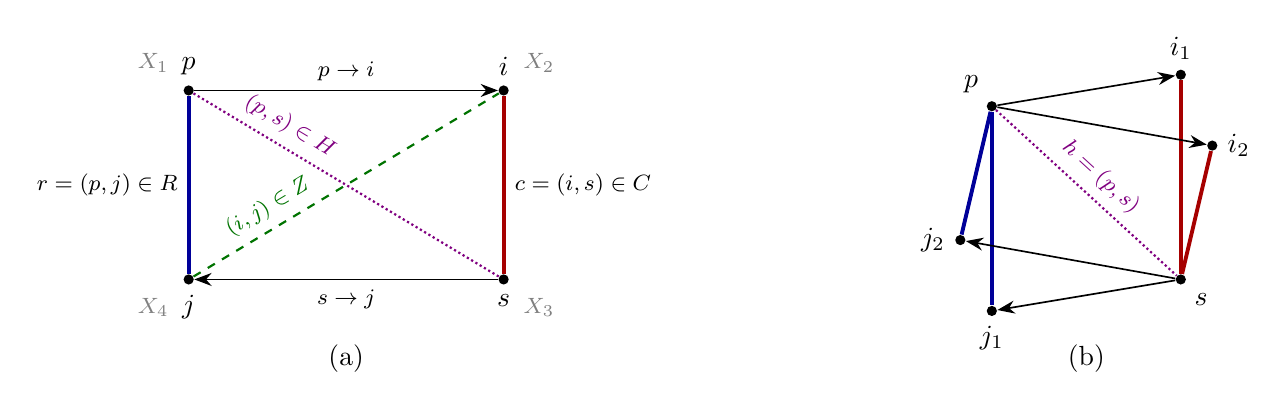
\begin{tikzpicture}[
  pt/.style={circle,fill,inner sep=1.3pt},
  arc/.style={-{Stealth[length=2.2mm]},semithick},
  memR/.style={line width=1.4pt,blue!60!black},
  memC/.style={line width=1.4pt,red!65!black},
  zdiag/.style={dashed,thick,green!45!black},
  hdiag/.style={densely dotted,thick,violet},
  set/.style={gray,font=\footnotesize},
  lab/.style={font=\footnotesize}]
  % (a) one conflict
  \node[pt,label=above:$p$] (p) at (0,2.4) {};
  \node[pt,label=above:$i$] (i) at (4,2.4) {};
  \node[pt,label=below:$s$] (s) at (4,0) {};
  \node[pt,label=below:$j$] (j) at (0,0) {};
  \node[set] at (-0.45,2.75) {$X_1$};
  \node[set] at (4.45,2.75) {$X_2$};
  \node[set] at (4.45,-0.35) {$X_3$};
  \node[set] at (-0.45,-0.35) {$X_4$};
  \draw[hdiag] (p) -- node[lab,pos=0.28,above,sloped] {$(p,s)\in H$} (s);
  \draw[zdiag] (j) -- node[lab,pos=0.28,above,sloped] {$(i,j)\in Z$} (i);
  \draw[memR] (p) -- node[lab,left,black] {$r=(p,j)\in R$} (j);
  \draw[memC] (i) -- node[lab,right,black] {$c=(i,s)\in C$} (s);
  \draw[arc] (p) -- node[lab,above] {$p\to i$} (i);
  \draw[arc] (s) -- node[lab,below] {$s\to j$} (j);
  \node at (2,-1.0) {(a)};
  % (b) a block R(h) x C(h), drawn with the half-turn symmetry
  \begin{scope}[xshift=9.6cm]
  \node[pt,label=above left:$p$] (bp) at (0.6,2.2) {};
  \node[pt,label=above:$i_1$] (bi1) at (3.0,2.6) {};
  \node[pt,label=right:$i_2$] (bi2) at (3.4,1.7) {};
  \node[pt,label=below right:$s$] (bs) at (3.0,0) {};
  \node[pt,label=below:$j_1$] (bj1) at (0.6,-0.4) {};
  \node[pt,label=left:$j_2$] (bj2) at (0.2,0.5) {};
  \draw[hdiag] (bp) -- node[lab,pos=0.5,above,sloped] {$h=(p,s)$} (bs);
  \draw[memR] (bp) -- (bj1);
  \draw[memR] (bp) -- (bj2);
  \draw[memC] (bi1) -- (bs);
  \draw[memC] (bi2) -- (bs);
  \draw[arc] (bp) -- (bi1);
  \draw[arc] (bp) -- (bi2);
  \draw[arc] (bs) -- (bj1);
  \draw[arc] (bs) -- (bj2);
  \node at (1.8,-1.0) {(b)};
  \end{scope}
\end{tikzpicture}
\caption{(a) A conflict between $r=(p,j)\in R$ and $c=(i,s)\in C$, covering the $Z$-point $(i,j)$ via $p\to i$ and $s\to j$. The involution $\sigma$ (defined below) acts as a half-turn of the square, exchanging $R$ with $C$ and $\alpha$ with $\beta$ while transposing both diagonals. (b) A conflict block $R(h)\times C(h)$ over $h=(p,s)$: every member $(p,j_b)\in R(h)$ conflicts with every member $(i_a,s)\in C(h)$, producing distinct $Z$-points $(i_a,j_b)$.}
\label{fig:conflict}
\end{figure}

If $r=(p,j)\in R$ and $c=(i,s)\in C$ cover the same point $z=(i,j)\in Z$, then $p\to i$ and $s\to j$, so $r$ and $c$ conflict. Since every $z\in Z$ arises from at least one conflict, it follows that any member of $R$ or $C$ covering a point in $Z$ must itself participate in a conflict. Moreover, if we define for each $h=(p,s)\in H$ the nonempty sets
\[
  R(h)=\{(p,j)\in R:\ s\to j\}\qquad\text{and}\qquad C(h)=\{(i,s)\in C:\ p\to i\},
\]
then the conflicts having $H$-point $h$ are precisely the pairs in the complete bipartite block $R(h)\times C(h)$ (see Figure~\ref{fig:conflict}(b)).

We associate with $\mathcal I$ four bipartite graphs, named after their two sides:
\begin{itemize}
\item $\Gamma_{HR}$ (between $H$ and $R$) and $\Gamma_{HC}$ (between $H$ and $C$), where $h\in H$ is adjacent to the members of $R(h)$ and $C(h)$, respectively;
\item $\Gamma_{RZ}$ (between $R$ and $Z$) and $\Gamma_{CZ}$ (between $C$ and $Z$), where a member of $R$ or $C$ is adjacent to the points of $Z$ that it covers.
\end{itemize}
Throughout, we write $\nu(\Gamma)$ for the maximum matching size in a bipartite graph $\Gamma$.

\begin{theorem}[Deletion lemma]\label{thm:deletion}
For every instance $\mathcal I$, there exist conflict-free subfamilies $R'\subseteq R$ and $C'\subseteq C$, retaining all members of $R$ and $C$ that participate in no conflicts, such that
\[
  \abs{R\setminus R'}+\abs{C\setminus C'}\le
  \min\{\nu(\Gamma_{HR}),\nu(\Gamma_{HC})\}+q\le\abs H+q,
\]
where $q$ is the number of points in $Z$ covered by no member of $R'$ or $C'$.
\end{theorem}

Theorem~\ref{thm:deletion} is used in Section~\ref{sec:extremal} and proved in Section~\ref{sec:proof}. Its proof uses the following symmetry. Instances come with an involution $\sigma$, the half-turn of the conflict square in Figure~\ref{fig:conflict}(a). Explicitly, given $\mathcal I=(X_1,X_2,X_3,X_4,\alpha,\beta,R,C)$, its dual instance is
\[
  \sigma(\mathcal I)=(X_3,X_4,X_1,X_2,\beta,\alpha,C^\T,R^\T),
\]
where $C^\T=\{(s,i):(i,s)\in C\}$ and $R^\T=\{(j,p):(p,j)\in R\}$.
Transposing coordinates identifies the conflicts, $Z$-points, and $H$-points of $\sigma(\mathcal I)$ with those of $\mathcal I$, while exchanging the roles of $R$ and $C$. In particular, $\Gamma_{HR}(\sigma(\mathcal I))\cong\Gamma_{HC}(\mathcal I)$, $\Gamma_{HC}(\sigma(\mathcal I))\cong\Gamma_{HR}(\mathcal I)$, and $\Gamma_{RZ}(\sigma(\mathcal I))\cong\Gamma_{CZ}(\mathcal I)$.


\section{The extremal argument}\label{sec:extremal}

By Lemmas~\ref{lem:deficit} and~\ref{lem:blowup} (with $m=n+1$), Theorem~\ref{thm:set} implies Theorem~\ref{thm:main}. The argument below is the extremal argument of~\cite{OAI}; we include it to keep the paper self-contained, and to show exactly which form of the deletion lemma is needed.

\begin{proof}[Proof of Theorem~\ref{thm:set}]
Suppose, for a contradiction, that $G$ is a nonempty oriented graph on $X=V(G)$ with minimum indegree at least one in which every nonempty proper subset $U\subsetneq X$ satisfies the strict concavity $\abs U+\abs{F^2(U)}<2\abs{F(U)}$, where $F=F_G$. Because every vertex has an in-neighbour, we have $F(X)=X$.

We apply the concavity to many subsets at once by working with subsets of $X\times X$. For any relation $\Omega\subseteq X\times X$, we define its column-wise and row-wise images under $F$ by
\[
  F_1\Omega=\{(i,j):\ (p,j)\in\Omega\text{ and }p\to i\}\qquad\text{and}\qquad
  F_2\Omega=\{(i,j):\ (i,s)\in\Omega\text{ and }s\to j\}.
\]
In other words, $F_1$ applies $F$ independently to each column $\Omega_{\ast j}=\{p:(p,j)\in\Omega\}$, whereas $F_2$ applies $F$ to each row $\Omega_{i\ast}=\{s:(i,s)\in\Omega\}$. We call a pair of relations $(P,Q)$ with $P,Q\subseteq X\times X$ \emph{compatible} if their one-step images are disjoint, that is, $F_1P\cap F_2Q=\varnothing$. Let $\Delta=\{(v,v):v\in X\}$ be the diagonal. The pair $(\Delta,\Delta)$ is compatible, as $(i,j)\in F_1\Delta\cap F_2\Delta$ would require both $j\to i$ and $i\to j$, impossible in an oriented graph. Among all compatible pairs $(P,Q)$ satisfying $\Delta\subseteq P\cap Q$, we choose one that maximizes the potential function
\[
  \Phi(P,Q)=\abs P+\abs Q+d,\qquad\text{where}\quad d=\abs X^2-\abs{F_1P}-\abs{F_2Q}.
\]
By compatibility, $d=\abs{X^2\setminus(F_1P\cup F_2Q)}$ counts the points of $X\times X$ lying outside both one-step images.

We first verify that every column of $P$ and every row of $Q$ is a nonempty proper subset of $X$. Since $\Delta\subseteq P\cap Q$, each column $P_{\ast j}$ contains $j$ and each row $Q_{i\ast}$ contains $i$. If $P_{\ast j}=X$ for some $j$, then $X\times\{j\}=F(X)\times\{j\}\subseteq F_1P$; picking any in-neighbour $w\to j$ in $G$ would then yield $(w,j)\in F_2\Delta\subseteq F_2Q$, contradicting $F_1P\cap F_2Q=\varnothing$. By symmetry, $Q_{i\ast}\subsetneq X$ for every $i$. We may therefore apply the strict concavity~\eqref{eq:concave} to each column $P_{\ast j}$ and each row $Q_{i\ast}$. Summing over all $j\in X$ and $i\in X$ gives
\[
  \abs P+\abs{F_1^2P}<2\abs{F_1P}\qquad\text{and}\qquad \abs Q+\abs{F_2^2Q}<2\abs{F_2Q}.
\]
Set $R=X^2\setminus F_2^2Q$ and $C=X^2\setminus F_1^2P$. The sum of these two inequalities is then a lower bound for $\abs R+\abs C$:
\begin{equation}\label{eq:gain}
  \abs R+\abs C=2\abs X^2-\abs{F_2^2Q}-\abs{F_1^2P}>\abs P+\abs Q+2d.
\end{equation}

These complements are the natural candidates for a better pair: besides~\eqref{eq:gain}, membership in $R$ and $C$ is what keeps the $H$-points of their conflicts away from $F_1P\cup F_2Q$, as we show below. The pair $(R,C)$ need not be compatible, however. Take $X_1=X_2=X_3=X_4=X$ and let $\alpha=\beta$ be the arc relation of $G$. Then $(R,C)$ is an instance in the sense of Section~\ref{sec:conflicts}, and by definition $F_1R\cap F_2C$ is its set $Z$ of $Z$-points. More generally, for $R'\subseteq R$ and $C'\subseteq C$, a point of $Z$ lies in $F_1R'\cup F_2C'$ if and only if some member of $R'$ or $C'$ covers it. Theorem~\ref{thm:deletion} provides conflict-free subfamilies $R'\subseteq R$ and $C'\subseteq C$ that retain all conflict-free members of $R$ and $C$ and satisfy
\begin{equation}\label{eq:del-applied}
  \abs{R\setminus R'}+\abs{C\setminus C'}\le\abs H+q,
\end{equation}
where $q$ is the number of points in $Z$ covered by no member of $R'$ or $C'$.

First, $\Delta\subseteq R\cap C$, and no diagonal member is in a conflict, so $\Delta\subseteq R'\cap C'$. Indeed, if $(v,v)\in F_2^2Q$, then $(v,s)\in F_2Q$ for some $s\to v$; but $(s,s)\in P$ gives $(v,s)\in F_1P$, contradicting compatibility. Likewise, a conflict between $(v,v)\in R$ and $(i,s)\in C$ would give $s\to v\to i$, and then $(s,s)\in P$ puts $(i,s)$ in $F_1^2P$, contradicting $(i,s)\in C$. Symmetrically, $\Delta\cap F_1^2P=\varnothing$ and no $(v,v)\in C$ is in a conflict.

Second, $\abs H\le d$. Consider any conflict between $(p,j)\in R$ and $(i,s)\in C$, which produces the $H$-point $(p,s)$ with $p\to i$ and $s\to j$. If $(p,s)$ belonged to $F_1P$, there would exist some $(u,s)\in P$ with $u\to p$; walking two steps along $u\to p\to i$ would then place $(i,s)$ in $F_1^2P$, contradicting $(i,s)\in C$. By the same token, if $(p,s)\in F_2Q$, there would exist $(p,t)\in Q$ with $t\to s$, and the two-step walk $t\to s\to j$ would place $(p,j)$ in $F_2^2Q$, contradicting $(p,j)\in R$. Consequently, $H$ is disjoint from $F_1P\cup F_2Q$, and so $\abs H\le d$.

Because $R'$ and $C'$ have no conflicts, we have $F_1R'\cap F_2C'=\varnothing$, so $(R',C')$ is a compatible pair with $\Delta\subseteq R'\cap C'$ and deletion cost $\abs{R\setminus R'}+\abs{C\setminus C'}\le\abs H+q\le d+q$. Let $d'=\abs X^2-\abs{F_1R'}-\abs{F_2C'}$ be the number of points outside $F_1R'\cup F_2C'$. As noted above, the $q$ uncovered points of $Z$ all lie outside $F_1R'\cup F_2C'$, ensuring that $q\le d'$. Combining this with~\eqref{eq:gain}, we arrive at
\[
  \Phi(R',C')=\abs{R'}+\abs{C'}+d'\ge\abs R+\abs C-(d+q)+d'
  \ge\abs R+\abs C-d>\abs P+\abs Q+d=\Phi(P,Q),
\]
which contradicts the extremal choice of $(P,Q)$.
\end{proof}


\section{Proof of the deletion lemma}\label{sec:proof}

The proof is by induction on $\abs R+\abs C$. Members in no conflict, and the case in which $H$ cannot be matched into one of the families, are handled by short reductions (Section~\ref{sec:reduce}). What remains is the case in which $H$ can be matched into both $R$ and $C$. There we delete everything, and the whole difficulty is the following inequality, proved in Section~\ref{sec:count}.

\subsection{Reduction to the counting lemma}\label{sec:reduce}

\begin{lemma}[Counting lemma]\label{lem:count}
Suppose that every member of $R$ and $C$ participates in a conflict, and that both $\Gamma_{HR}$ and $\Gamma_{HC}$ possess matchings saturating $H$. Then $\abs R+\abs C\le\abs Z+\abs H$.
\end{lemma}

\begin{proof}[Proof of Theorem~\ref{thm:deletion}, assuming Lemma~\ref{lem:count}]
We proceed by induction on $\abs R+\abs C$, calling any pair $(R',C')$ satisfying the conclusion of the theorem a \emph{solution}. If there are no conflicts, then $\nu(\Gamma_{HR})=\nu(\Gamma_{HC})=0$ and $(R,C)$ itself is a solution. Assume henceforth that at least one conflict exists, and set $\nu^\ast=\min\{\nu(\Gamma_{HR}),\nu(\Gamma_{HC})\}$.

Removing a member that is in no conflict changes none of $Z$, $H$, $\nu^\ast$, and such a member covers no point of $Z$ (Section~\ref{sec:conflicts}); so adding it back to a solution of the smaller instance, which exists by induction, gives a solution.

We may therefore assume that every member of $R$ and $C$ participates in at least one conflict. Suppose next that $\nu^\ast<\abs H$. By applying the involution $\sigma$ if necessary (which exchanges $R$ and $C$ while preserving $\abs R+\abs C$, $\nu^\ast$, and $q$), we may assume without loss of generality that $\nu(\Gamma_{HR})=\nu^\ast<\abs H$. By the defect form of Hall's theorem, there exists a nonempty subset $H'\subseteq H$ whose neighbourhood $R_{H'}=\bigcup_{h\in H'}R(h)$ in $\Gamma_{HR}$ satisfies
\[
  \abs{R_{H'}}\le\abs{H'}-\abs H+\nu^\ast.
\]
Because each block $R(h)$ is nonempty, so is $R_{H'}$. We may thus apply the induction hypothesis to the instance $(R\setminus R_{H'},C)$, whose sets of $Z$-points, $H$-points, and uncovered $Z$-points we denote by $Z^\circ$, $H^\circ$, and $q^\circ$. This gives conflict-free subfamilies $R'\subseteq R\setminus R_{H'}$ and $C'\subseteq C$ satisfying
\[
  \abs{(R\setminus R_{H'})\setminus R'}+\abs{C\setminus C'}
  \le\abs{H^\circ}+q^\circ.
\]
(Since every member of the original instance now lies in a conflict, the requirement that $(R',C')$ retain the conflict-free members of the original instance is vacuous, here and in the final case below.)
Plainly $Z^\circ\subseteq Z$ and $H^\circ\subseteq H$. No $h\in H'$ can survive in $H^\circ$, because every conflict with $H$-point $h$ involves a member of $R(h)\subseteq R_{H'}$, all of which have been deleted; hence $\abs{H^\circ}\le\abs H-\abs{H'}$. Moreover, any point of $Z^\circ$ left uncovered by $R'$ and $C'$ is also a point of $Z$ left uncovered by $R'$ and $C'$, so $q^\circ\le q$. Combining these estimates gives
\[
  \abs{R\setminus R'}+\abs{C\setminus C'}
  =\abs{R_{H'}}+\abs{(R\setminus R_{H'})\setminus R'}+\abs{C\setminus C'}
  \le\abs{R_{H'}}+\abs H-\abs{H'}+q\le\nu^\ast+q,
\]
so $(R',C')$ is a solution.

Finally, suppose that every member participates in a conflict and $\nu^\ast=\abs H$, so that both $\Gamma_{HR}$ and $\Gamma_{HC}$ admit matchings saturating $H$. In this case we delete everything by setting $R'=C'=\varnothing$. Then all points of $Z$ are left uncovered ($q=\abs Z$), and Lemma~\ref{lem:count} guarantees that the total deletion cost is $\abs R+\abs C\le\abs H+\abs Z=\nu^\ast+q$.
\end{proof}


\subsection{Greedy bases in transversal matroids}\label{sec:greedy}

For subsets $S\subseteq X_3$ and $Q\subseteq X_4$, let $\lambda(S,Q)$ denote the maximum size of a matching in the bipartite subgraph of $\beta$ induced between $S$ and $Q$, and write $N_\beta(S)=\{j\in X_4:s\to j\text{ for some }s\in S\}$. By K\H{o}nig's theorem (or Hall's marriage theorem~\cite{Hall}), this matching number is given by the min-cut formula
\[
  \lambda(S,Q)=\min_{M\subseteq S}\bigl(\abs{S\setminus M}+\abs{N_\beta(M)\cap Q}\bigr).
\]
If $M_1,M_2$ attain the minimum for $(S_1,Q_1)$ and $(S_2,Q_2)$, then $M_1\cup M_2$ and $M_1\cap M_2$ are admissible for $(S_1\cup S_2,Q_1\cap Q_2)$ and $(S_1\cap S_2,Q_1\cup Q_2)$; since $N_\beta(M_1\cap M_2)\subseteq N_\beta(M_1)\cap N_\beta(M_2)$, this shows that $\lambda$ is \emph{bisubmodular}: for all $S_1,S_2\subseteq X_3$ and $Q_1,Q_2\subseteq X_4$,
\begin{equation}\label{eq:bisub}
  \lambda(S_1,Q_1)+\lambda(S_2,Q_2)\ \ge\
  \lambda(S_1\cup S_2,\,Q_1\cap Q_2)+\lambda(S_1\cap S_2,\,Q_1\cup Q_2).
\end{equation}
For any $S\subseteq X_3$, $T\subseteq X_4$, and $j\in X_4\setminus T$, the marginal matching increment
\[
  \partial_j(S,T)=\lambda(S,T\cup\{j\})-\lambda(S,T)\in\{0,1\}
\]
satisfies, by~\eqref{eq:bisub} (with $S_1=S_2=S$, $Q_1=T\cup\{j\}$, $Q_2=T'$, respectively $(S_1,Q_1)=(S,T)$, $(S_2,Q_2)=(S',T\cup\{j\})$),
\begin{equation}\label{eq:mono}
  \partial_j(S,T)\ge\partial_j(S,T')\quad(T\subseteq T'\subseteq X_4\setminus\{j\})
  \qquad\text{and}\qquad
  \partial_j(S',T)\ge\partial_j(S,T)\quad(S\subseteq S'\subseteq X_3).
\end{equation}
We call the first inequality \emph{diminishing returns}. Also $\lambda(S,T)=\lambda(S,T\cap N_\beta(S))$, since vertices outside $N_\beta(S)$ are isolated. For fixed $S$, $Q\mapsto\lambda(S,Q)$ is the rank function of the transversal matroid on $X_4$ determined by $\beta$ and $S$.

Fix once and for all a global linear order $\prec$ on $X_4$, and for any $Q\subseteq X_4$ and $j\in X_4$ write $Q_{\succ j}=\{x\in Q:j\prec x\}$. The \emph{greedy set} of $Q$ with respect to $S$, that is, the basis of $Q$ in this matroid obtained by scanning $Q$ in decreasing $\prec$-order, is
\[
  g(S,Q)=\{j\in Q:\ \partial_j(S,Q_{\succ j})=1\}.
\]

\begin{lemma}[Greedy bases]\label{lem:greedy}
For every $S\subseteq X_3$ and $Q\subseteq X_4$, we have $\abs{g(S,Q)}=\lambda(S,Q)$, and $g(S,Q)$ can be completely matched into $S$ (that is, $\lambda(S,Q_0)=\abs{Q_0}$ for every $Q_0\subseteq g(S,Q)$).
\end{lemma}

\begin{proof}
Telescoping the marginal increments along $\prec$ gives $\lambda(S,Q)=\sum_{j\in Q}\partial_j(S,Q_{\succ j})=\abs{g(S,Q)}$. Writing $J=g(S,Q)$, we have $J_{\succ j}\subseteq Q_{\succ j}$ for each $j\in J$, so diminishing returns~\eqref{eq:mono} gives $\partial_j(S,J_{\succ j})\ge\partial_j(S,Q_{\succ j})=1$. Summing over $j\in J$ yields $\lambda(S,J)=\sum_{j\in J}\partial_j(S,J_{\succ j})=\abs J$, so $J$, and hence every $Q_0\subseteq J$, can be completely matched into $S$.
\end{proof}


\subsection{Proof of the counting lemma}\label{sec:count}

The counting lemma combines two inequalities. The first shows, via Hall's theorem and double counting, that when $H$ can be matched into $C$, the family $R$ can be matched into $Z$.

\begin{lemma}[Local Hall lemma]\label{lem:local}
If every member of $R$ participates in at least one conflict and $\Gamma_{HC}$ contains a matching saturating $H$, then $\Gamma_{RZ}$ contains a matching saturating $R$.
\end{lemma}

\begin{proof}
For fixed $j$, we weight each member $r\in U$ and each point $z\in T$ (both defined below) by the number of vertices $s$ with $s\to j$ through which it can take part in a conflict. The matching saturating $H$ shows that $T$ carries at least as much total weight as $U$, while passing from a member to an adjacent point cannot increase the weight; for a minimal Hall violator these two facts, together with the positive weight of every member, are incompatible.

The graph $\Gamma_{RZ}$ decomposes over $j\in X_4$ as the disjoint union of the bipartite graphs $\Gamma_{RZ}^j$ between the $j$-fibres of $R$ and $Z$. Fix $j\in X_4$ and write $N_j$ for neighbourhoods in $\Gamma_{RZ}^j$. By Hall's marriage theorem, it suffices to show that $\abs{N_j(U)}\ge\abs U$ for every subset $U$ of members $(p,j)\in R$. Suppose, for a contradiction, that some subset violates Hall's condition, and choose a violator $U$ of minimum cardinality, with $T=N_j(U)$. By minimality, for every $w\in U$ the subset $U\setminus\{w\}$ satisfies Hall's condition and thus admits a saturating matching into $T$. This forces $\abs T=\abs U-1$ and provides, for each $w\in U$, a bijection $\mu_w\colon U\setminus\{w\}\to T$ with $\mu_w(r)\in N_j(r)$ for all $r\in U\setminus\{w\}$.

Let $S_j=\{s\in X_3:s\to j\}$. For each $s\in S_j$, define
\[
  U_s=\{(p,j)\in U:\ p\to i\text{ for some }(i,s)\in C\}\qquad\text{and}\qquad
  T_s=\{(i,j)\in T:\ (i,s)\in C\}.
\]
If $(p,j)\in U_s$ and $(i,s)\in C$ with $p\to i$, then $(p,j)$ and $(i,s)$ conflict (since $s\to j$), yielding $(p,s)\in H$ and $(i,j)\in T_s$. A matching in $\Gamma_{HC}$ saturating $H$ maps the distinct $H$-points $\{(p,s):(p,j)\in U_s\}$ injectively to members $(i,s)\in C$ with $p\to i$, and hence to distinct points $(i,j)\in T_s$. Thus $\abs{U_s}\le\abs{T_s}$ for every $s\in S_j$. Summing this inequality over all $s\in S_j$ and interchanging the order of summation gives
\begin{equation}\label{eq:sumcount}
  \sum_{r\in U}a_r\le\sum_{z\in T}b_z,\qquad\text{where}\quad
  a_r=\abs{\{s\in S_j:r\in U_s\}},\quad b_z=\abs{\{s\in S_j:z\in T_s\}}.
\end{equation}
On the other hand, whenever $r=(p,j)\in U$ is adjacent to $z=(i,j)\in T$ in $\Gamma_{RZ}^j$, we have $p\to i$, which implies that every $s\in S_j$ satisfying $z\in T_s$ also satisfies $r\in U_s$; consequently, $a_r\ge b_z$. Fixing any $w\in U$ and pairing $U\setminus\{w\}$ with $T$ via the bijection $\mu_w$, we find
\[
  \sum_{r\in U}a_r=a_w+\sum_{r\in U\setminus\{w\}}a_r\ge a_w+\sum_{r\in U\setminus\{w\}}b_{\mu_w(r)}=a_w+\sum_{z\in T}b_z.
\]
Finally, since every member of $R$ participates in a conflict, $w=(p,j)$ must conflict with some $(i,s)\in C$, which ensures $s\in S_j$ and $w\in U_s$, so $a_w\ge 1$. This contradicts~\eqref{eq:sumcount}.
\end{proof}

The second inequality, Lemma~\ref{lem:rank} below, comes from linear algebra. Assign an independent indeterminate $x_{pi}$ to each arc $p\to i$ and $y_{sj}$ to each arc $s\to j$, and work over the rational function field $\mathbb K$ generated by these indeterminates. Consider the four incidence matrices $L\in\mathbb K^{Z\times R}$, $N\in\mathbb K^{C\times Z}$, $B\in\mathbb K^{H\times R}$, and $A\in\mathbb K^{C\times H}$ defined by setting $L_{(i,j),(p,j)}=x_{pi}$ and $A_{(i,s),(p,s)}=x_{pi}$ whenever $p\to i$, setting $N_{(i,s),(i,j)}=y_{sj}$ and $B_{(p,s),(p,j)}=y_{sj}$ whenever $s\to j$, and setting all other entries to $0$. A direct check shows that both matrix products $NL$ and $AB$ have $((i,s),(p,j))$-entry equal to $x_{pi}y_{sj}$ if $(p,j)$ and $(i,s)$ conflict, and $0$ otherwise; thus the conflict matrix factors through both $Z$ and $H$ as
\[
  NL=AB.
\]
The matrices $L$, $N$, and $B$ are block-diagonal (decomposing over $j\in X_4$, $i\in X_2$, and $p\in X_1$, respectively) with distinct indeterminates appearing in each block. By a theorem of Edmonds~\cite{Edmonds}, their generic ranks over $\mathbb K$ coincide with the maximum matching numbers $\nu(\Gamma_{RZ})$, $\nu(\Gamma_{CZ})$, and $\nu(\Gamma_{HR})$. Applying Sylvester's rank inequality to $NL=AB$ therefore yields
\[
  \nu(\Gamma_{RZ})+\nu(\Gamma_{CZ})-\abs Z=\rank L+\rank N-\abs Z\le\rank(NL)=\rank(AB)\le\rank B=\nu(\Gamma_{HR}).
\]
We now prove this inequality without matrices.

\begin{lemma}[Combinatorial Sylvester inequality]\label{lem:rank}
For every instance $\mathcal I$, we have
\[
  \nu(\Gamma_{RZ})+\nu(\Gamma_{CZ})\le\abs Z+\nu(\Gamma_{HR})\le\abs Z+\abs H.
\]
\end{lemma}

\begin{proof}
For each $i\in X_2$, define the slices $C_i=\{s\in X_3:(i,s)\in C\}$ and $Z^i=\{j\in X_4:(i,j)\in Z\}$; similarly, for each $p\in X_1$, set $R_p=\{j\in X_4:(p,j)\in R\}$ and $C^{(p)}=\bigcup_{i:\,p\to i}C_i$. First, if $p\to i$, then $R_p\cap N_\beta(C_i)\subseteq Z^i$, because any $j\in R_p$ and $s\in C_i$ with $s\to j$ produce a conflict between $(p,j)\in R$ and $(i,s)\in C$ with $Z$-point $(i,j)$. Second, $\Gamma_{CZ}$ decomposes as the disjoint union over $i\in X_2$ of the bipartite graphs induced by $\beta$ between $C_i$ and $Z^i$, so that $\nu(\Gamma_{CZ})=\sum_{i\in X_2}\lambda(C_i,Z^i)$.

For each $i\in X_2$, let $J_i=g(C_i,Z^i)\subseteq Z^i$ be the greedy set along $\prec$, and form the combined set $Y=\{(i,j)\in Z:j\in J_i\}$. By Lemma~\ref{lem:greedy}, we have $\abs Y=\sum_i\abs{J_i}=\nu(\Gamma_{CZ})$. Let $W$ denote the set of members $(p,j)\in R$ that cover at least one point $(i,j)\in Y$ (meaning $p\to i$ and $j\in J_i$).

Every member $(p,j)\in R\setminus W$ is adjacent in $\Gamma_{RZ}$ exclusively to points of $Z\setminus Y$; thus any matching in $\Gamma_{RZ}$ uses at most $\abs{Z\setminus Y}=\abs Z-\abs Y$ edges incident to $R\setminus W$ and at most $\abs W$ edges incident to $W$, giving
\[
  \nu(\Gamma_{RZ})\le\abs W+\abs Z-\abs Y=\abs W+\abs Z-\nu(\Gamma_{CZ}).
\]
Since $\nu(\Gamma_{HR})\le\abs H$ holds trivially, it remains only to show that $W$ can be completely matched into $H$ in $\Gamma_{HR}$, which will give $\abs W\le\nu(\Gamma_{HR})$.

The difficulty is that a member $(p,j)\in W$ may cover points of $Y$ in several rows $i$ with $p\to i$, and matchings chosen independently in different rows could send two members $(p,j)$ and $(p,j')$ to the same $s\in X_3$, that is, to the same $H$-point $(p,s)$. Choosing every $J_i$ greedily along one fixed order prevents this: an element that is greedy for $C_i$ stays greedy for the union $C^{(p)}$ of the rows met by $p$, so for each $p$ the relevant elements are independent in a single transversal matroid and can be matched at once.

To construct such a matching, fix $p\in X_1$ and consider the slice $W_p=\{j\in X_4:(p,j)\in W\}\subseteq R_p$. For any $j\in W_p$, we can choose $i\in X_2$ with $p\to i$ and $j\in J_i$. Setting $T=(R_p)_{\succ j}$, we have $T\cap N_\beta(C_i)\subseteq Z^i_{\succ j}$ since $R_p\cap N_\beta(C_i)\subseteq Z^i$. Moreover, $j\in J_i\subseteq Z^i$ implies $j\in N_\beta(C_i)$. Using diminishing returns, the isolation of vertices outside $N_\beta(C_i)$, and the second inequality in~\eqref{eq:mono} for $C_i\subseteq C^{(p)}$, we obtain the chain of inequalities
\[
  1=\partial_j(C_i,Z^i_{\succ j})\le\partial_j(C_i,T\cap N_\beta(C_i))
  =\partial_j(C_i,T)\le\partial_j(C^{(p)},T)\le 1.
\]
Hence $\partial_j(C^{(p)},(R_p)_{\succ j})=1$, which means that $W_p\subseteq g(C^{(p)},R_p)$. Lemma~\ref{lem:greedy} therefore supplies an injection $\phi_p\colon W_p\to C^{(p)}$ such that $\phi_p(j)\to j$ for every $j\in W_p$. By definition of $C^{(p)}$, for each $j\in W_p$ the image $s=\phi_p(j)$ lies in $C_{i'}$ for some $i'$ with $p\to i'$; the resulting conflict between $(p,j)\in R$ and $(i',s)\in C$ shows that $(p,s)\in H$ and $(p,j)\in R(p,s)$. Assembling the assignments $(p,j)\mapsto(p,\phi_p(j))$ across all $p\in X_1$ and $j\in W_p$ produces a matching in $\Gamma_{HR}$ saturating $W$, completing the proof.
\end{proof}

\begin{proof}[Proof of Lemma~\ref{lem:count}]
Lemma~\ref{lem:local} applied directly to $\mathcal I$ gives $\nu(\Gamma_{RZ})=\abs R$. Applying Lemma~\ref{lem:local} to the dual instance $\sigma(\mathcal I)$ (where $\Gamma_{HC}(\sigma(\mathcal I))\cong\Gamma_{HR}(\mathcal I)$ likewise has a matching saturating its $H$-points) yields $\nu(\Gamma_{CZ}(\mathcal I))=\nu(\Gamma_{RZ}(\sigma(\mathcal I)))=\abs C$. The desired bound now follows from Lemma~\ref{lem:rank}.
\end{proof}

\begin{remark}\label{rem:oai}
Theorem~\ref{thm:deletion} also yields a sharpening of the auxiliary matching bound in~\cite{OAI}. Let $\Gamma$ be the bipartite graph with left part $R\sqcup Z_L$ and right part $C\sqcup Z_R$ (where $Z_L,Z_R$ are disjoint copies of $Z$), with edges joining conflicting pairs $(r,c)\in R\times C$, as well as $r\in R$ to $z_R\in Z_R$ and $z_L\in Z_L$ to $c\in C$ whenever $r$ or $c$ covers $z\in Z$. Given a solution $(R',C')$ from Theorem~\ref{thm:deletion}, form a vertex set $K$ in $\Gamma$ by taking all deleted members $(R\setminus R')\cup(C\setminus C')$, the copies $z_R$ of points $z\in Z$ covered by $R'$, and the copies $z_L$ of points $z\in Z$ covered by $C'$. Since $R'$ and $C'$ are conflict-free, no $z\in Z$ is covered by both $R'$ and $C'$, so $\abs K=\abs{R\setminus R'}+\abs{C\setminus C'}+\abs Z-q\le\abs Z+\min\{\nu(\Gamma_{HR}),\nu(\Gamma_{HC})\}$. By construction, $K$ is a vertex cover of $\Gamma$, which implies $\nu(\Gamma)\le\abs K\le\abs Z+\min\{\nu(\Gamma_{HR}),\nu(\Gamma_{HC})\}$, refining the bound $\nu(\Gamma)\le\abs Z+\abs H$ of~\cite{OAI}.
\end{remark}


\section{Consequences}\label{sec:consequences}

We conclude with two consequences of Theorem~\ref{thm:main}. The second is well known to follow from the conjecture (Remark~\ref{rem:ch}); we include the short deductions for completeness. See also Seacrest~\cite{Seacrest2015} for a related arc-weighted formulation.

\begin{corollary}[Vertex-weighted form]\label{cor:weighted}
For every nonempty oriented graph $D$ and every weight function $w\colon V(D)\to[0,\infty)$, there exists a vertex $v\in V(D)$ such that $w(N_1^+(v))\le w(N_2^+(v))$, where $w(S)=\sum_{x\in S}w(x)$.
\end{corollary}

\begin{proof}
Suppose first that $w$ takes positive integer values. Construct a blow-up oriented graph $D_w$ by replacing each vertex $u\in V(D)$ with an independent set $I_u=\{(u,k):1\le k\le w(u)\}$ of size $w(u)$, and directing an arc from $(u,k)$ to $(y,l)$ whenever $u\to y$ in $D$. Because $D$ has no digons, for any vertex $x=(v,k)$ in $D_w$ we have $N_1^+(x)=\bigcup_{u\in N_1^+(v)}I_u$ and $N_2^+(x)=\bigcup_{u\in N_2^+(v)}I_u$. Applying Theorem~\ref{thm:main} to $D_w$ therefore yields a vertex $v\in V(D)$ with $w(N_1^+(v))\le w(N_2^+(v))$. By scaling, the same holds for all positive rational weight functions, and a standard compactness (closedness) argument extends the conclusion to all $w\in[0,\infty)^{V(D)}$.
\end{proof}

\begin{corollary}[Directed triangles]\label{cor:triangle}
Every oriented graph $D$ on $n\ge1$ vertices with no directed triangle contains a vertex $v$ satisfying $2\abs{N_1^+(v)}+\abs{N_1^-(v)}\le n-1$, where $N_1^-(v)=\{u\in V(D):u\to v\}$. Consequently, any oriented graph on $n\ge1$ vertices with minimum outdegree and minimum indegree at least $n/3$ contains a directed triangle.
\end{corollary}

\begin{proof}
By Theorem~\ref{thm:main}, $D$ contains a good vertex $v$. Since $D$ is oriented and triangle-free, $N_2^+(v)$ cannot intersect $N_1^-(v)$ (as any $w\in N_2^+(v)\cap N_1^-(v)$ would close a two-step walk $v\to u\to w$ into a directed triangle $v\to u\to w\to v$). Thus the four sets $\{v\}$, $N_1^+(v)$, $N_1^-(v)$, and $N_2^+(v)$ are pairwise disjoint, which gives
\[
  \abs{N_1^+(v)}\le\abs{N_2^+(v)}\le n-1-\abs{N_1^+(v)}-\abs{N_1^-(v)}.
\]
Rearranging gives $2\abs{N_1^+(v)}+\abs{N_1^-(v)}\le n-1$, which is violated whenever all in- and out-degrees are at least $n/3$.
\end{proof}

\begin{remark}\label{rem:ch}
The Caccetta--H\"aggkvist conjecture~\cite{CH} asserts in particular that every digraph on $n$ vertices with minimum outdegree at least $n/3$ contains a directed cycle of length at most three; for oriented graphs, a directed triangle. Seymour observed that his conjecture implies the weaker version in which both the minimum outdegree and the minimum indegree are at least $n/3$ (see~\cite{CSY,Sullivan}); this is the second statement of Corollary~\ref{cor:triangle}. This semidegree version was listed as open in Sullivan's survey~\cite{Sullivan}. The outdegree version remains open to our knowledge; the best bound known is due to Hladk\'y, Kr\'al', and Norin~\cite{HKN}, who showed that minimum outdegree at least $0.3465n$ forces a directed triangle.
\end{remark}

\begin{thebibliography}{99}
\raggedright
\bibitem{BBKS}
J.~Brantner, G.~Brockman, B.~Kay and E.~Snively, Contributions to Seymour's
second neighborhood conjecture, \emph{Involve} 2 (2009), no.~4, 387--395,
\url{https://doi.org/10.2140/involve.2009.2.387}.

\bibitem{CH}
L.~Caccetta and R.~H\"aggkvist, On minimal digraphs with given girth,
\emph{Congressus Numerantium} 21 (1978), 181--187.

\bibitem{CSY}
G.~Chen, J.~Shen and R.~Yuster, Second neighborhood via first neighborhood
in digraphs, \emph{Ann. Comb.} 7 (2003), no.~1, 15--20,
\url{https://doi.org/10.1007/s000260300001}.

\bibitem{DL}
N.~Dean and B.~J.~Latka, Squaring the tournament---an open problem,
\emph{Congressus Numerantium} 109 (1995), 73--80.

\bibitem{Edmonds}
J.~Edmonds, Systems of distinct representatives and linear algebra,
\emph{J. Res. Nat. Bur. Standards Sect. B} 71B (1967), 241--245,
\url{https://doi.org/10.6028/jres.071B.033}.

\bibitem{EGGK}
A.~Espuny D\'iaz, A.~Gir\~ao, B.~Granet and G.~Kronenberg, Seymour's second
neighbourhood conjecture: random graphs and reductions, \emph{Random
Structures Algorithms} 66 (2025), no.~1, e21251,
\url{https://doi.org/10.1002/rsa.21251}.

\bibitem{FY}
D.~Fidler and R.~Yuster, Remarks on the second neighborhood problem,
\emph{J. Graph Theory} 55 (2007), no.~3, 208--220,
\url{https://doi.org/10.1002/jgt.20229}.

\bibitem{Fisher}
D.~C.~Fisher, Squaring a tournament: a proof of Dean's conjecture,
\emph{J. Graph Theory} 23 (1996), 43--48,
\url{https://doi.org/10.1002/(SICI)1097-0118(199609)23:1<43::AID-JGT4>3.0.CO;2-K}.

\bibitem{Ghazal}
S.~Ghazal, Seymour's second neighborhood conjecture for tournaments
missing a generalized star, \emph{J. Graph Theory} 71 (2012), no.~1, 89--94,
\url{https://doi.org/10.1002/jgt.20634}.

\bibitem{Hall}
P.~Hall, On representatives of subsets,
\emph{J. London Math. Soc.} 10 (1935), 26--30,
\url{https://doi.org/10.1112/jlms/s1-10.37.26}.

\bibitem{HT}
F.~Havet and S.~Thomass\'e, Median orders of tournaments: a tool for the
second neighborhood problem and Sumner's conjecture,
\emph{J. Graph Theory} 35 (2000), 244--256,
\url{https://doi.org/10.1002/1097-0118(200012)35:4<244::AID-JGT2>3.0.CO;2-H}.

\bibitem{HKN}
J.~Hladk\'y, D.~Kr\'al' and S.~Norin, Counting flags in triangle-free digraphs,
\emph{Combinatorica} 37 (2017), no.~1, 49--76,
\url{https://doi.org/10.1007/s00493-015-2662-5}.

\bibitem{HP}
H.~Huang and F.~Peng, An improved bound on Seymour's second neighborhood
conjecture, arXiv:2412.20234, 2024,
\url{https://arxiv.org/abs/2412.20234}.

\bibitem{KL}
Y.~Kaneko and S.~C.~Locke, The minimum degree approach for Paul Seymour's
distance 2 conjecture, \emph{Congressus Numerantium} 148 (2001), 201--206.

\bibitem{OAI}
OpenAI, A proof of Seymour's second-neighborhood conjecture, preprint in the
OpenAI Math Release, September 23, 2026,
\href{https://github.com/openai/math/blob/main/preprints/A-proof-of-Seymours-second-neighborhood-conjecture-September-23-2026/paper.pdf}{\nolinkurl{github.com/openai/math}}.

\bibitem{Seacrest2015}
T.~Seacrest, The arc-weighted version of the second neighborhood conjecture,
\emph{J. Graph Theory} 78 (2015), no.~3, 219--228,
\url{https://doi.org/10.1002/jgt.21800}.

\bibitem{Seacrest2019}
T.~Seacrest, Seymour's second neighborhood conjecture for subsets of
vertices, arXiv:1808.06293v3, revised April 12, 2019,
\url{https://arxiv.org/abs/1808.06293v3}.

\bibitem{Sullivan}
B.~D.~Sullivan, A summary of results and problems related to the
Caccetta--H\"aggkvist conjecture, arXiv:math/0605646, 2006,
\url{https://arxiv.org/abs/math/0605646}.
\end{thebibliography}

\end{document}